\documentclass[UTF8,a4paper,10pt]{ctexart}
\usepackage[left=2.50cm, right=2.50cm, top=2.50cm, bottom=2.50cm]{geometry}
%页边距
\CTEXsetup[format={\Large\bfseries}]{section} %设置章标题居左

%%%%%%%%%%%%%%%%%%%%%%%
% -- text font --
% compile using Xelatex
%%%%%%%%%%%%%%%%%%%%%%%
% -- 中文字体 --
%\setmainfont{Microsoft YaHei}  % 微软雅黑
%\setmainfont{YouYuan}  % 幼圆    
%\setmainfont{NSimSun}  % 新宋体
%\setmainfont{KaiTi}    % 楷体
%\setmainfont{SimSun}   % 宋体
%\setmainfont{SimHei}   % 黑体
% -- 英文字体 --
%\usepackage{times}
%\usepackage{mathpazo}
%\usepackage{fourier}
%\usepackage{charter}

%\usepackage{helvet}

\usepackage{amsmath, amsfonts, amssymb} % math equations, symbols
\usepackage[english]{babel}
\usepackage{color}	% color content
\usepackage{graphicx}	% import figures
\usepackage{url}	% hyperlinks
\usepackage{bm} 	% bold type for equations
\usepackage{multirow}
\usepackage{booktabs}
\usepackage{epstopdf}
\usepackage{epsfig}
\usepackage{algorithm}
\usepackage{algorithmic}
\usepackage{listings}
\usepackage{xcolor}
\usepackage{booktabs}
\usepackage{zhnumber}
\usepackage{longtable}
\usepackage{subfigure}
\usepackage{float}
\usepackage{caption}
\usepackage{subfigure}
\renewcommand\thesection{\zhnum{section}}
\renewcommand \thesubsection {\arabic{section}}
\renewcommand{\algorithmicrequire}{ \textbf{Input:}}
% use Input in the format of Algorithm  
\renewcommand{\algorithmicensure}{ \textbf{Initialize:}}
% use Initialize in the format of Algorithm  
\renewcommand{\algorithmicreturn}{ \textbf{Output:}}
% use Output in the format of Algorithm  
%%%%%%%%%%%%%%%%%%
\usepackage{listings}
\usepackage{color}
\definecolor{dkgreen}{rgb}{0,0.6,0}
\definecolor{gray}{rgb}{0.5,0.5,0.5}
\definecolor{mauve}{rgb}{0.58,0,0.82}
\lstset{frame=tb,
  language=Python,
  aboveskip=3mm,
  belowskip=3mm,
  showstringspaces=false,
  columns=flexible,
  basicstyle={\small\ttfamily},
  numbers=left,%设置行号位置none不显示行号
  %numberstyle=\tiny\courier, %设置行号大小
  numberstyle=\tiny\color{gray},
  keywordstyle=\color{blue},
  commentstyle=\color{dkgreen},
  stringstyle=\color{mauve},
  breaklines=true,
  breakatwhitespace=true,
  escapeinside=``,%逃逸字符(1左面的键),用于显示中文例如在代码中`中文...`
  tabsize=4,
  extendedchars=false %解决代码跨页时,章节标题,页眉等汉字不显示的问题
}

%%%%%%%%%%%%%%%%%%%%%%%%%%%%
\usepackage{fancyhdr} %设置页眉、页脚
\pagestyle{fancy}
\lhead{}
\chead{}
%\rhead{\includegraphics[width=1.2cm]{fig/ZJU_BLUE.eps}}
\lfoot{}
\cfoot{}
\rfoot{}
\fancyfoot[RE,RO]{~\thepage~}

\fancyhead[RE,RO]{计算物理导论 \quad 2022春季学期 \quad 作业8  \quad 何翼成}

%%%%%%%%%%%%%%%%%%%%%%%
%  设置水印
%%%%%%%%%%%%%%%%%%%%%%%
%\usepackage{draftwatermark}         % 所有页加水印
%\usepackage[firstpage]{draftwatermark} % 只有第一页加水印
% \SetWatermarkText{Water-Mark}           % 设置水印内容
% \SetWatermarkText{\includegraphics{fig/ZJDX-WaterMark.eps}}         % 设置水印logo
% \SetWatermarkLightness{0.9}             % 设置水印透明度 0-1
% \SetWatermarkScale{1}                   % 设置水印大小 0-1    

\usepackage{hyperref} %bookmarks
\hypersetup{colorlinks, bookmarks, unicode} %unicode

\title{\textbf{差分法求解偏微分方程}}
\author{ 何翼成 \thanks{学号:520072910043; \newline
    邮箱地址:heyicheng@sjtu. edu. cn} }
\date{\today}

\begin{document}
\maketitle

%\begin{abstract}
%这是一篇中文小论文。这个部分用来写摘要。摘要的章标题默认是英文,还没找到改成中文的方法:(
%\end{abstract}
\section*{Project 1}
\section{题目分析}
%%%以下为插入图片模板
%\quad \newline
	\begin{figure}[!htbp]
		\centering
		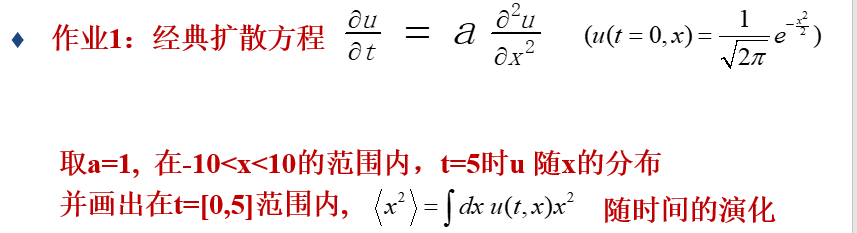
\includegraphics[width=1\textwidth,height=0.2\textwidth]{pictures/project1.png}
		\caption{题目总览} \label{project1}
	\end{figure}


\section{代码展示}


\lstset{language=matlab}
\begin{lstlisting}
  %project1
  clear;clc;
  dx=0.05;
  dt=0.001;
  x=-10:dx:10;
  t=0:dt:5;
  r=dt/(dx^2);
  
  %偏微分方程的初始条件以及边界条件
  numX=length(x)-1;
  numT=length(t)-1;
  Phi=ones(numT+1,numX+1);
  Phi(1,:)=1/sqrt(2*pi)*exp(-x.^2/2);%初始条件
  Phi(2:numT+1,1)=0;%边界条件
  Phi(2:numT+1,numX+1)=0;%边界条件
  
  %差分法计算数值解
  for k=1:numT
      for i=2:numX
          Phi(k+1,i)=(1-2*r)*Phi(k,i)+r*(Phi(k,i-1)+Phi(k,i+1));
      end
  end
  
  %绘制(x,t,Phi)的三维网格图
  figure(1)
  set(gcf,'units','normalized','position',[0.2 0.2 0.6 0.6]);
  [xx,tt]=meshgrid(x,t);
  mesh(xx,tt,Phi)
  xlabel('x')
  ylabel('t')
  zlabel('\Phi(x,t)')
  figure(2)
  plot(x,Phi(end,:),'k')
  xlabel('x')
  ylabel('\Phi at t=5')
  
  %计算<x^2>的时间变化
  for ti=1:numT+1
      X2(ti)=sum(Phi(ti,:).*x.^2*dx);
  end
  figure(3)
  plot(t,X2,'r')
  xlabel('t')
  ylabel('<x^2> at t \in [0,5]')
\end{lstlisting}

\section{结果分析与结论}
通过上述的代码可以完整得到u(x,t)在$x\in[-10,10]\times t\in [0,5]$的演化情况,为了进行分析进行截取即可。
首先是t=5的部分,显然我们对所命名的二维数组截取(end,:)即可。

	\begin{figure}[!htbp]
		\centering
		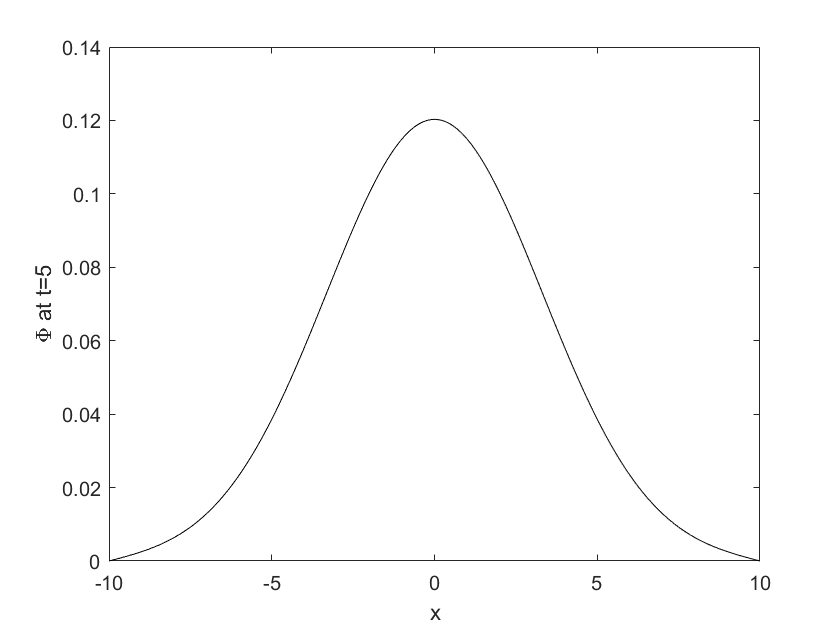
\includegraphics[width=0.5\textwidth,height=0.4\textwidth]{pictures/result1.png}
		\caption{t=5时的\phi 在x\in [-10,10]的分布} \label{p1}
	\end{figure}

  然后就是计算的方均值。我们可以按照时间顺序依次截取u(x,t),然后按照离散数列求和的方法计算得到积分值,
  最后依次绘制在二维图像上即可。\newline

  \begin{figure}[!htbp]
		\centering
		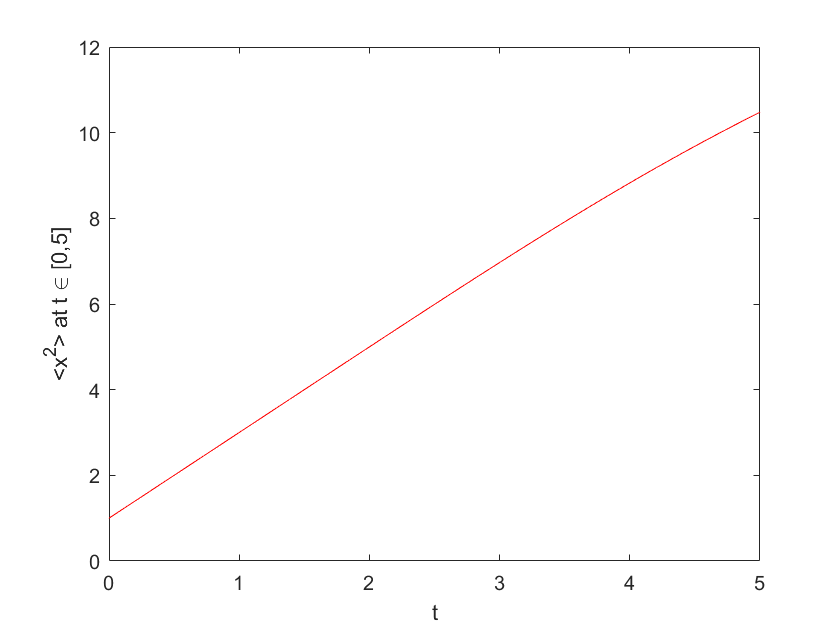
\includegraphics[width=0.5\textwidth,height=0.4\textwidth]{pictures/result2.png}
		\caption{<x^2>在t\in[0,5]的演化过程} \label{p2}
	\end{figure}

最后展示以下求解得到的总览值。\newline

  \begin{figure}[!htbp]
		\centering
		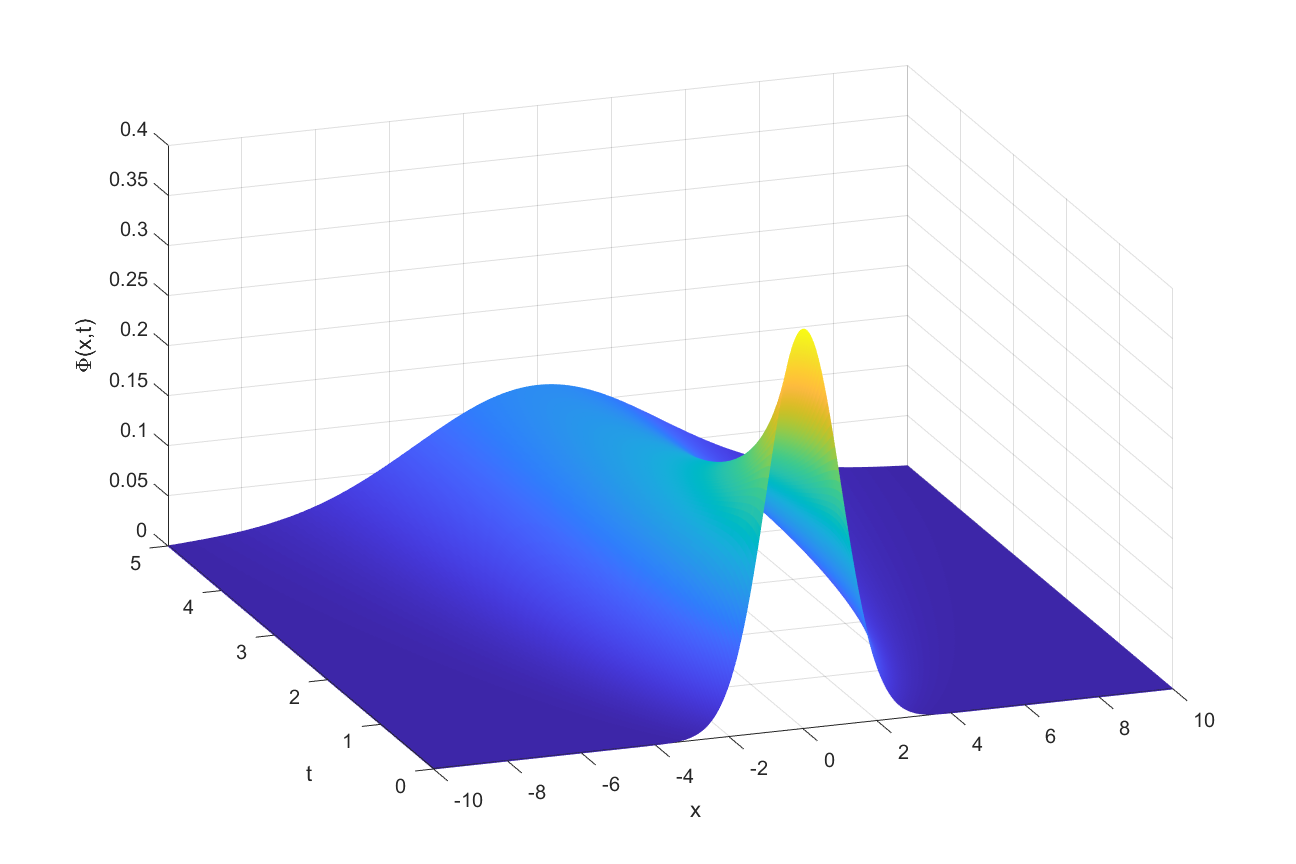
\includegraphics[width=0.5\textwidth,height=0.4\textwidth]{pictures/result3.png}
		\caption{u(x,t)在X,T平面上的演化总览} \label{p3}
	\end{figure}


  %%%%%%%%%%%%%%%%%%%%%%%%%第二题%%%%%%%%%%%%%%%%%%%%%%%%%%%%%%%%%
  %%%%%%%%%%%%%%%%%%%%%%%%%第二题%%%%%%%%%%%%%%%%%%%%%%%%%%%%%%%%%
  %%%%%%%%%%%%%%%%%%%%%%%%%第二题%%%%%%%%%%%%%%%%%%%%%%%%%%%%%%%%%
  %%%%%%%%%%%%%%%%%%%%%%%%%第二题%%%%%%%%%%%%%%%%%%%%%%%%%%%%%%%%%
\section*{Project2}
\section{题目分析}
\begin{figure}[!htbp]
  \centering
  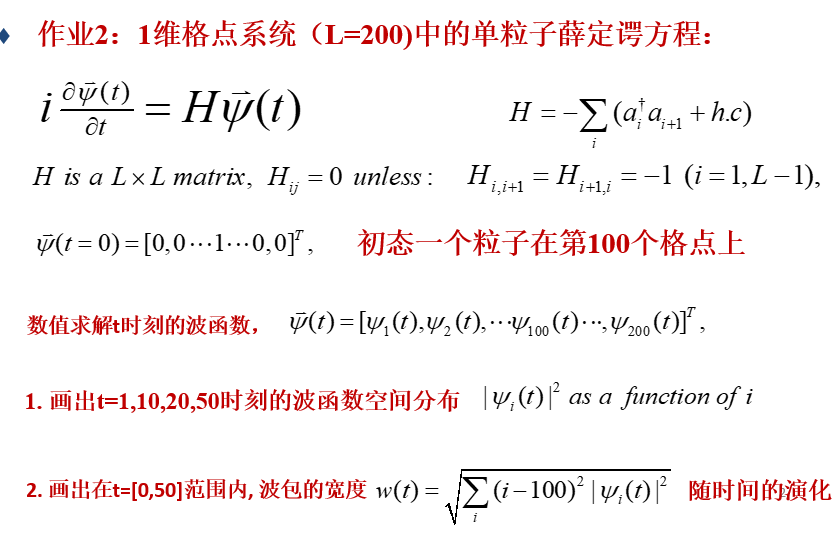
\includegraphics[width=0.7\textwidth,height=0.55\textwidth]{pictures/project2.png}
  \caption{题目总览} \label{project2}
\end{figure}
由题意知我们可以将$\frac{\partial \psi(t)}{\partial t}$差分化,
从而将该方程离散写作$i\frac{\psi_{i+1}-\psi_{i}}{\Delta t}=H\psi_{i}$,
其中$H$为题目中所定义的对称矩阵。所以我们将不难看出,这个题目实际上是迭代的
背景。\newline


\section{代码展示}
~\\
\lstset{language=matlab}
\begin{lstlisting}
  %%
  %project2
  clear;clc;
  L=200;
  dt=0.001;
  %哈密顿矩阵的生成
  H=zeros(L,L);
  for ii=1:L-1
      H(ii,ii+1)=-1;
      H(ii+1,ii)=-1;
  end
  psi=zeros(200,1);
  psi(100)=1;
  numT=50/dt+1;
  psi_series=zeros(L,numT);
  psi_series(:,1)=psi;
  for n=2:numT
      psi_series(:,n)=psi_series(:,n-1)-1i*H*psi_series(:,n-1)*dt;
  end
  %计算波函数的模方
  psi2_series=abs(psi_series);
  figure(1)%t=1,10,20,50的情况
  ts=[1,10,20,50];
  for tn=1:length(ts)
  tmp=ts(tn);
  subplot(2,2,tn)
  l=ts(tn)/dt;
  plot(1:L,psi2_series(:,tmp/dt+1)')
  xlabel("i \in [1,L] with t="+tmp)
  xlim([1,200])
  ylabel("|\Psi|^2(i)")
  end
  %计算波包宽度
  b=((1:L)'-100).^2;
  w=zeros(1,numT);
  for j=1:numT
      w(j)=sqrt(sum(b.*psi2_series(:,j)));
  end
  figure(2)%绘制波包宽度随时间的演化
  tspan=linspace(0,50,numT);
  plot(tspan,w,'k')
  xlabel('t')
  ylabel('w(t)')
\end{lstlisting}

\section{结果分析与结论}
下面展示的是t在不同时间的时候$|\psi(t)|^2$在$i\in [1,200]$的分布,如图已经标注了各个子图所代表的时间。\newline

	\begin{figure}[!htbp]
		\centering
		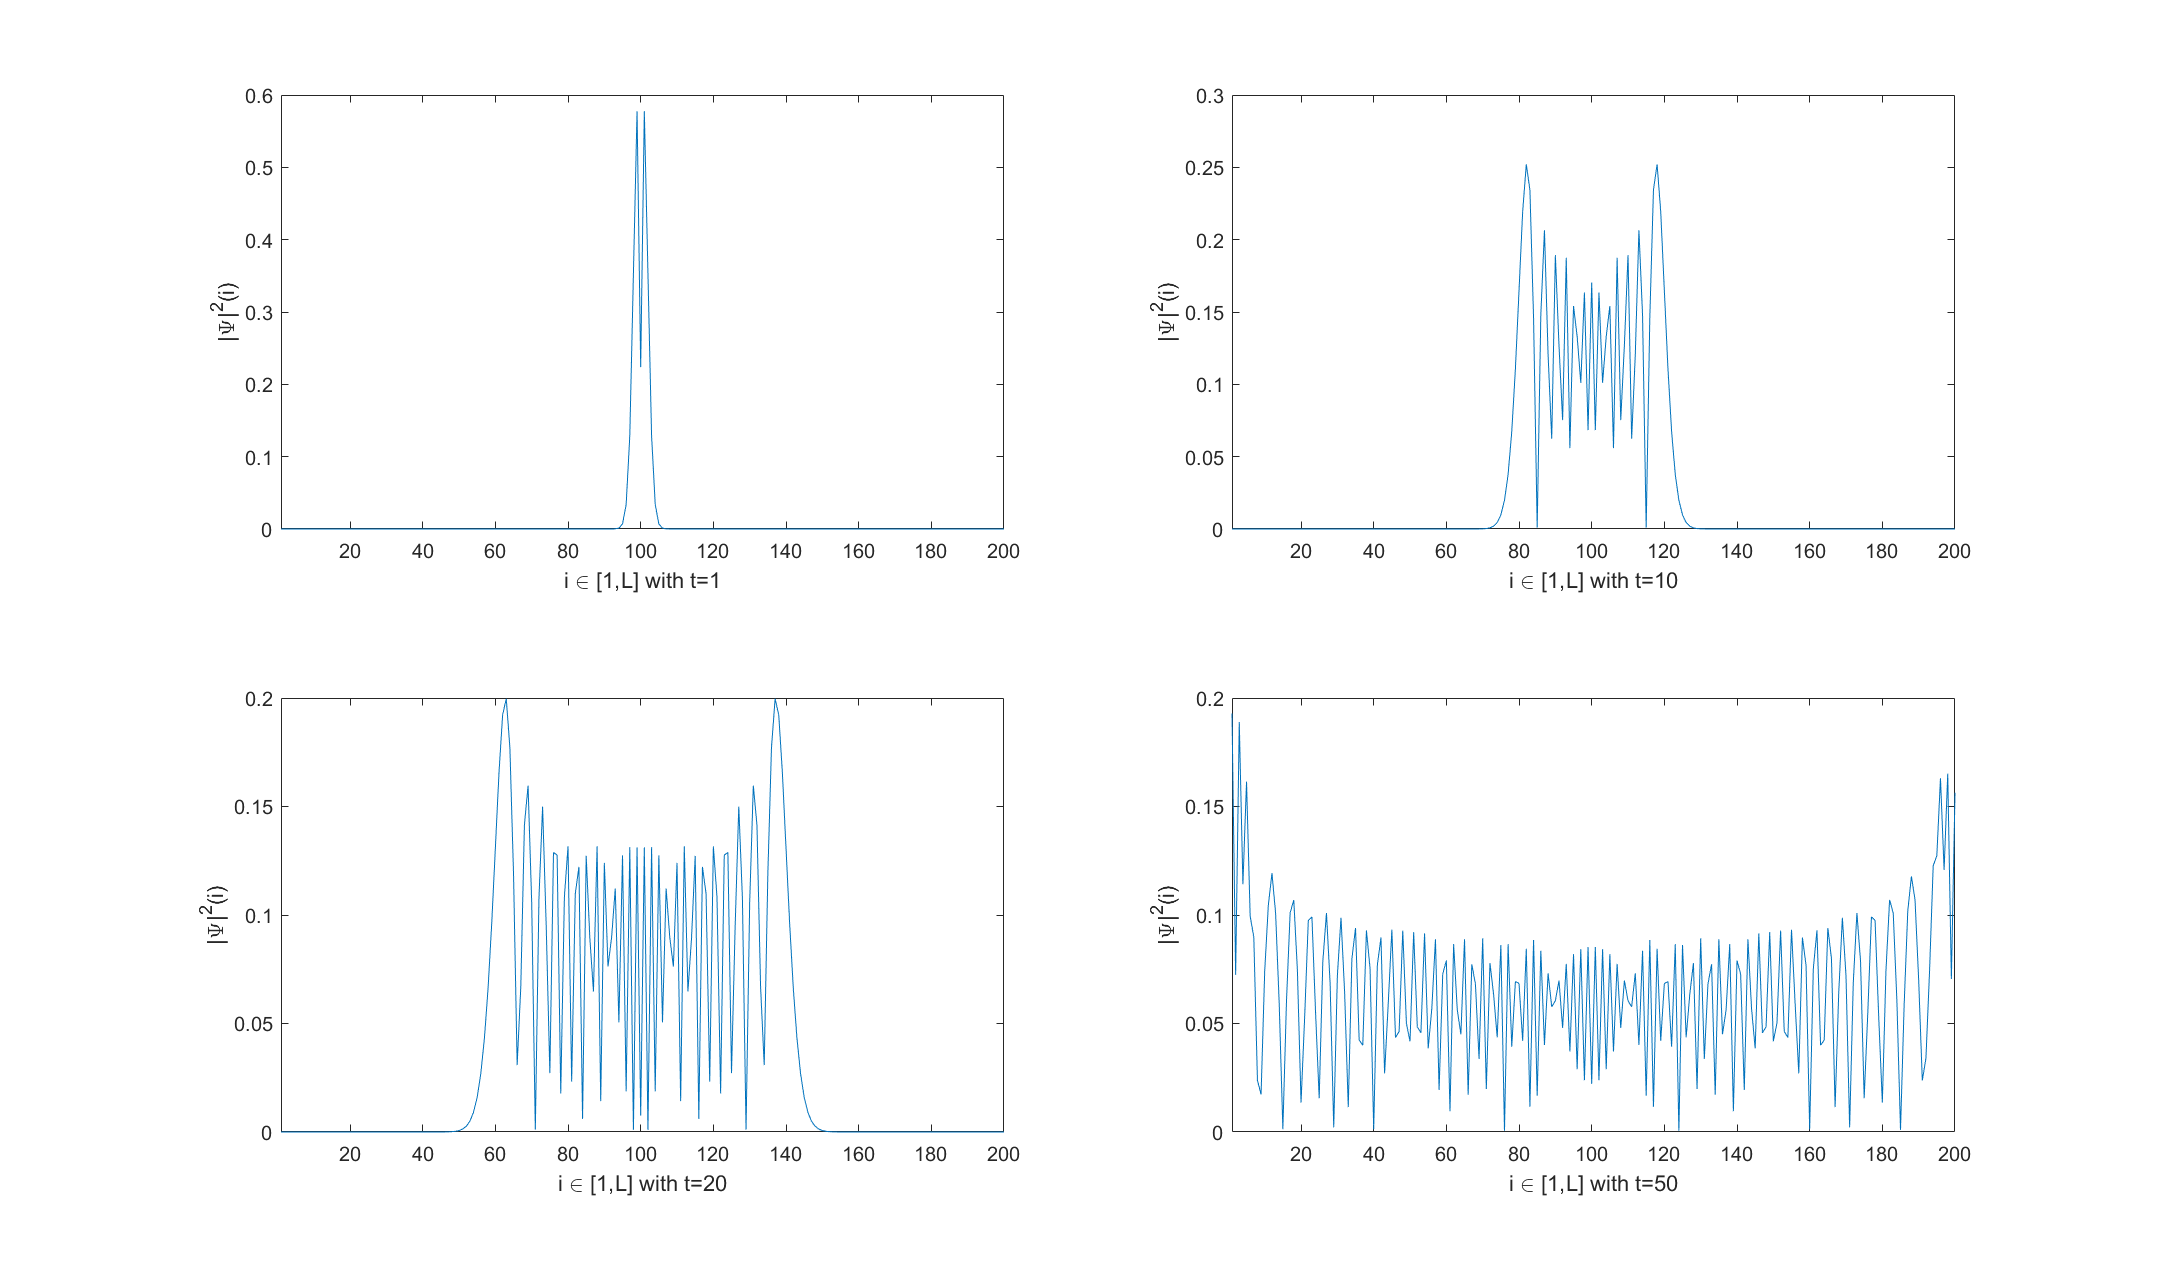
\includegraphics[width=1\textwidth,height=0.6\textwidth]{pictures/psi2.png}
		\caption{不同时间下的|\psi|^2} \label{psi2}
	\end{figure}

  下面展示的是$w(t)$在$t\in [0,50]$的演化情况,可以看出随着时间的延长波包的宽度逐渐增大,在本数值方法下t接近50的时候,$w(t)$出现了小幅度的回落。\newline


	\begin{figure}[!htbp]
		\centering
		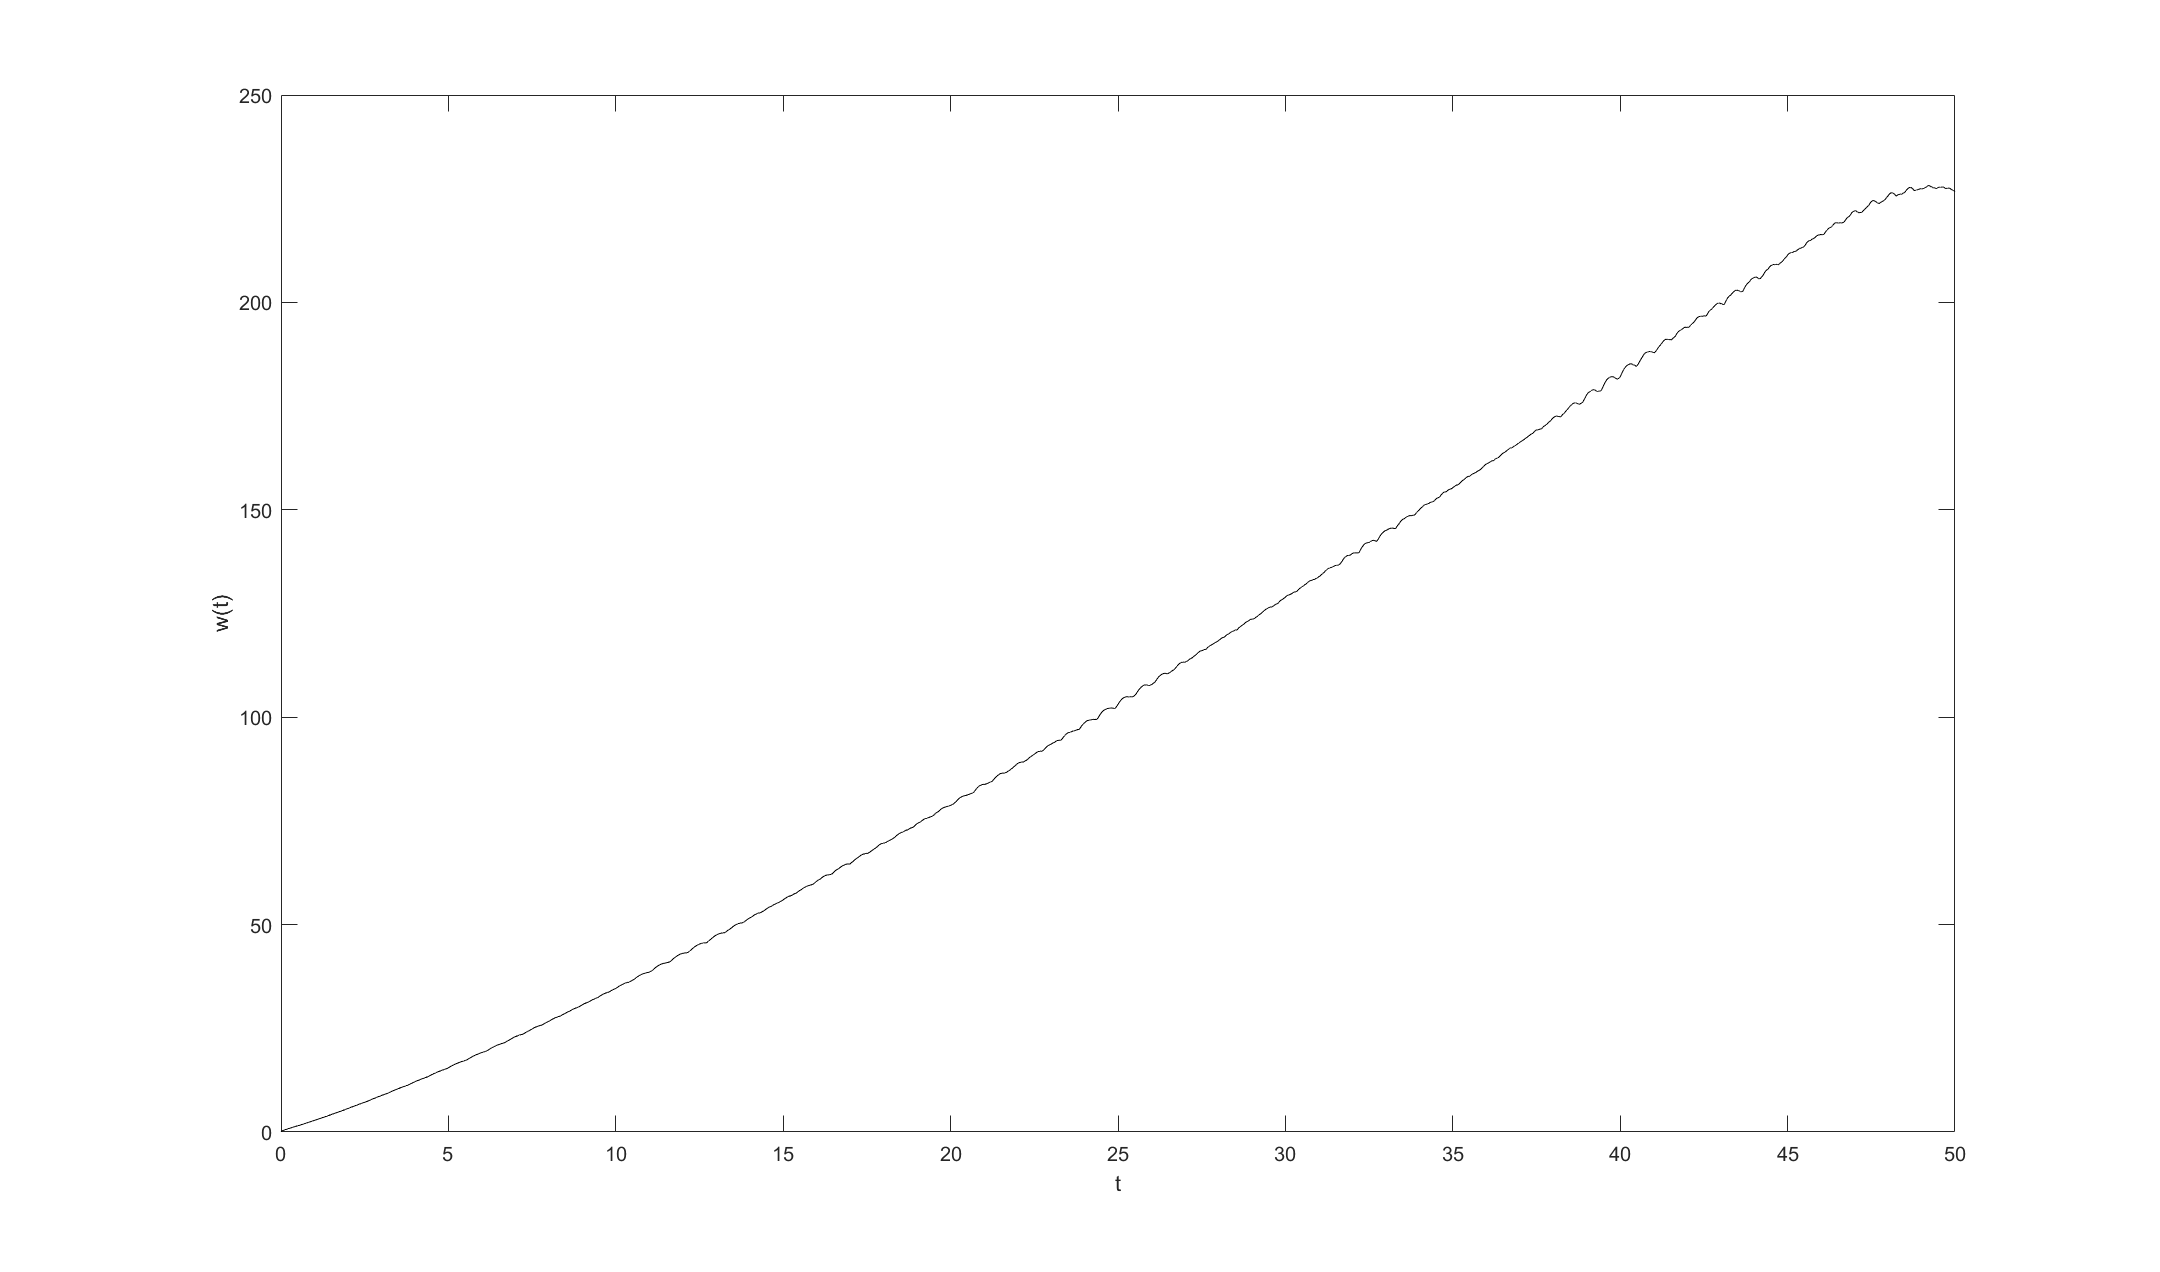
\includegraphics[width=0.6\textwidth,height=0.4\textwidth]{pictures/wt.png}
		\caption{波包宽度w(t)随着时间的演化情况} \label{wt}
	\end{figure}
%以下为插入代码模板
%~\\
%\lstset{language=matlab}
%\begin{lstlisting}
%\end{lstlisting}


%%%以下为插入图片模板
%\quad \newline
%	\begin{figure}[!htbp]
%		\centering
%		\includegraphics[width=0.5\textwidth,height=0.375\textwidth]{pictures/minscale.png}
%		\caption{最小风向} \label{minsacle}
%	\end{figure}

%%%以下为插入图片模板
%\quad \newline
%	\begin{figure}[!htbp]
%		\centering
%		\includegraphics[width=0.5\textwidth,height=0.375\textwidth]{pictures/minscale.png}
%		\caption{最小风向} \label{minsacle}
%	\end{figure}

%    \begin{algorithm}
%		\caption{Title of the Algorithm}
%     	\begin{algorithmic}[1]
%			\REQUIRE some words.  % this command shows "Input"
%			\ENSURE ~\\           % this command shows "Initialized"
%			some text goes here ... \\
%			\WHILE {\emph{not converged}}
%			\STATE ... \\  % line number at left side
%			\ENDWHILE
%			\RETURN this is the lat part.  % this command shows "Output"
%		\end{algorithmic}
%	\end{algorithm}

\end{document}